%
\documentclass[11pt]{article}

% The usual packages
\usepackage{booktabs}
\usepackage{array}
\usepackage{subcaption}

\usepackage{fullpage}
\usepackage{breakcites}
\usepackage{setspace}
\usepackage{endnotes}
%\usepackage{float} % can't use with floatrow
\usepackage{amsmath}
\usepackage{amsfonts}
\usepackage{amssymb}
\usepackage{rotating}
\usepackage{longtable}
\usepackage{microtype}
\usepackage{graphicx}
\usepackage{hyperref}
%\usepackage[usenames,dvipsnames]{color}
\usepackage{url}
\usepackage{natbib}
\usepackage{framed}
\usepackage{epigraph}
\usepackage{lipsum}
\usepackage{textcomp} % for \textrightarrow
\usepackage{dcolumn}
%\restylefloat{table}
\bibpunct{(}{)}{;}{a}{}{,}

% Set paragraph spacing the way I like
\parskip=0pt
\parindent=20pt

%\usepackage{helvet}
%\usepackage[labelfont={bf}, margin=0cm, font=small, skip=0pt]{caption}

\newcommand\numberthis{\addtocounter{equation}{1}\tag{\theequation}}

% Define mathematical results
\newtheorem{lemma}{Lemma}
\newtheorem{proposition}{Proposition}
\newtheorem{theorem}{Theorem}
\newtheorem{claim}{Claim}
\newenvironment{proof}[1][Proof]{\begin{trivlist}
\item[\hskip \labelsep {\bfseries #1}]}{\end{trivlist}}
\newenvironment{definition}[1][Definition]{\begin{trivlist}
\item[\hskip \labelsep {\bfseries #1}]}{\end{trivlist}}
\newenvironment{example}[1][Example]{\begin{trivlist}
\item[\hskip \labelsep {\bfseries #1}]}{\end{trivlist}}
\newenvironment{remark}[1][Remark]{\begin{trivlist}
\item[\hskip \labelsep {\bfseries #1}]}{\end{trivlist}}
\DeclareMathOperator*{\argmin}{arg\,min}
\DeclareMathOperator{\med}{med}
\DeclareMathOperator*{\E}{\text{E}}
%\DeclareMathOperator*{\Pr}{\text{Pr}}

%Set up fonts the way I like
%\usepackage{tgpagella}
%\usepackage[T1]{fontenc}
%\usepackage[bitstream-charter]{mathdesign}

%% Baskervald
%\usepackage[lf]{Baskervaldx} % lining figures
%\usepackage[bigdelims,vvarbb]{newtxmath} % math italic letters from Nimbus Roman
%\usepackage[cal=boondoxo]{mathalfa} % mathcal from STIX, unslanted a bit
%\renewcommand*\oldstylenums[1]{\textosf{#1}}

%\usepackage[T1]{fontenc}
%\usepackage{newtxtext,newtxmath}

% A special command to create line break in table cells
\newcommand{\specialcell}[2][c]{%
 \begin{tabular}[#1]{@{}c@{}}#2\end{tabular}}

%% Set up lists the way I like
% Redefine the first level
\renewcommand{\theenumi}{\arabic{enumi}.}
\renewcommand{\labelenumi}{\theenumi}
% Redefine the second level
\renewcommand{\theenumii}{\alph{enumii}.}
\renewcommand{\labelenumii}{\theenumii}
% Redefine the third level
\renewcommand{\theenumiii}{\roman{enumiii}.}
\renewcommand{\labelenumiii}{\theenumiii}
% Redefine the fourth level
\renewcommand{\theenumiv}{\Alph{enumiv}.}
\renewcommand{\labelenumiv}{\theenumiv}
% Eliminate spacing around lists
\usepackage{enumitem}
\setlist{nolistsep}

% Create footnote command so that my name
% has an asterisk rather than a one.
\long\def\symbolfootnote[#1]#2{\begingroup%
\def\thefootnote{\fnsymbol{footnote}}\footnote[#1]{#2}\endgroup}
%\usepackage{footmisc}
%\renewcommand{\thefootnote}{\symbolfootnote{footnote}}

% Create the colors I want
\usepackage{color, xcolor}
\definecolor{color1}{RGB}{217,95,2}  % orange
\definecolor{color2}{RGB}{27,158,119}  % green
\definecolor{color3}{RGB}{117,112,179}  % purple

% for colored \left( and \right)
\newcommand{\cleft}[2][.]{%
  \begingroup\colorlet{savedleftcolor}{.}%
  \color{#1}\left#2\color{savedleftcolor}%
}
\newcommand{\cright}[2][.]{%
  \color{#1}\right#2\endgroup
}

% for drawing arrows
\usepackage{tikz}
\usetikzlibrary{calc,shapes}

\newcommand{\tikzmark}[1]{\tikz[overlay,remember picture] \node (#1) {};}
\newcommand{\DrawBox}[2]{%
  \begin{tikzpicture}[overlay,remember picture]
    \draw[->,shorten >= 6pt, shorten <= 2pt, out=-90, in=90, distance=1.2cm, color2, thick] (MarkA.east) to (MarkB.east);
    \draw[->,shorten >= 6pt, shorten <= 2pt, out=-90, in=90, distance=1cm, color2, thick] (MarkC.west) to (MarkD.east);
  \end{tikzpicture}
}

% remarks by equations
\newcommand{\justif}[2]{&{#1}&\text{#2}}


% set up pdf
\hypersetup{
pdftitle={}, % title
pdfauthor={Carlisle Rainey}, % author
pdfkeywords={bias} {first difference} {marginal effect} {quantities of interest} {maximum likelihood}
pdfnewwindow=true, % links in new window
colorlinks=true, % false: boxed links; true: colored links
linkcolor=black, % color of internal links
citecolor=black, % color of links to bibliography
filecolor=blue, % color of file links
urlcolor=blue % color of external links
}

% section headers
%\usepackage[scaled]{helvet}
%\renewcommand\familydefault{\sfdefault}
%\usepackage[T1]{fontenc}
%\usepackage{titlesec}
%\titleformat{\section}
%  {\normalfont\sffamily\Large\bfseries}
%  {\thesection}{1em}{}
%\titleformat{\subsection}
%  {\normalfont\sffamily\large\bfseries}
%  {\thesection}{1em}{}
%  \titleformat{\subsubsection}
%  {\normalfont\sffamily\bfseries}
%  {\thesection}{1em}{}

% enable comments in pdf
\newcommand{\dtk}[1]{\textcolor{blue}{#1}}
\newcommand{\ctk}[1]{\textcolor{red}{#1}}

\begin{document}

\begin{center}

{\Large \textbf{Simulation-Induced Bias in Quantities of Interest}}\symbolfootnote[1]{All computer code necessary for replication is available on \href{https://github.com/carlislerainey/unnecessary}{GitHub}. Thanks to audiences at Florida State University and the 2018 Texas Methods Meeting for helpful discussions. Christopher Gandrud, Michael Hanmer, Justin Kirkland, Thomas Leeper, Matthew Pietryka, and Christopher Wlezien offered valuable feedback on earlier versions.}

\vspace{1cm}

Carlisle Rainey\symbolfootnote[2]{Carlisle Rainey is Associate Professor of Political Science, Florida State University, 540 Bellamy, Tallahassee, FL, 32306. (\href{mailto:crainey@fsu.com}{crainey@fsu.com}).}

\vspace{5mm}

Holger L. Kern\symbolfootnote[3]{Holger L. Kern is Assistant Professor of Political Science, Florida State University, 541 Bellamy, Tallahassee, FL, 32306. (\href{mailto:hkern@fsu.edu}{hkern@fsu.edu}).}

\vspace{1cm}

\today
\end{center}

\vspace{5mm}

% Abstract
{\centerline{\textbf{Abstract}}}
\begin{quote}\noindent
Following \cite{KingTomzWittenberg2000} researchers commonly obtain point estimates of quantities of interest by simulating model coefficients, transforming these simulated coefficients into simulated quantities of interest, and then taking the average of the simulated quantities of interest.
In contrast, other researchers directly transform coefficient estimates into quantities of interest, using the invariance property of maximum likelihood estimators.
These approaches are not equivalent.
We show both analytically and empirically that computing quantities of interest using the average of simulations can introduce substantial bias.
Instead, researchers should use the invariance property to calculate the maximum likelihood estimates of their quantities of interest.
\\
\end{quote}

% Add quote to first page
% \epigraph{}

%\begin{center}
%Manuscript word count:
%\end{center}

% Remove page number from first page
\thispagestyle{empty}

% Start main text
%\newpage
%\doublespace
\onehalfspace
%\section*{Introduction}



% political scientists use ML estimators, but the coefs are not always informative
Political scientists employ maximum likelihood (ML) estimators to model a wide variety of dependent variables.
Examples include logit and probit models for binary outcomes; ordered logit and probit models for ordered categorical outcomes; multinomial logit and probit models for unordered categorical outcomes; Poisson and negative binomial regression for count data; and beta regression for fractions.
Political scientists propose several ML estimators and researchers regularly use these estimators in political science research (e.g., \citealt{Nagler1994}, \citealt{KatzKing1999}; \citealt{Mebane2000}).
Many of these models have coefficients that do not directly interest substantive researchers.
Instead, researchers usually need to transform the coefficients to compute substantively-meaningful quantities of interest.


% introduce KTW and QIs;
% HOLGER: I've restored the earlier longer discussion. I think we want to give more credit to King et al.; one of them or one of their students or co-authors is probably going to be a reviewer
\cite{KingTomzWittenberg2000} dramatically improves the reporting of quantitative research by urging researchers to focus on substantively meaningful quantities of interest such as predicted probabilities, expected counts, marginal effects, and first differences.
Prior to the publication of \cite{KingTomzWittenberg2000} and the availability of easy-to-use software for Stata (CLARIFY) and \texttt{R} (Zelig), political science research commonly reported lengthy tables of coefficient estimates and paid little or no attention to the substantive interpretation of the estimates beyond their sign and statistical significance.

The citations demonstrate the impact of King, Tomz, and Wittenberg (2000) on the literature.
According to the Web of Science, by January 2018 \cite{KingTomzWittenberg2000} has received 1,097 citations, making it the fourth most-cited methodology article in political science, at least among those published in the \textit{American Political Science Review}, the \textit{American Journal of Political Science}, and \textit{Political Analysis}.
Moreover, their paper has received the second most-citations overall in the \textit{American Journal of Political Science}, falling just $56$ citations short of \cite{BeckKatzTucker1998}.
Google Scholar lists 3,598 citations for \cite{KingTomzWittenberg2000}, 1,437 citations for \cite{TomzWittenbergKing2003} (which provides an overview of the CLARIFY software), and 318 citations for Imai, King, and Lau (2008) (which proposes a common framework for statistical analysis and software development centered on Zelig).
In short, the advice that \cite{KingTomzWittenberg2000} offers noticeably improves research in political science and the social sciences more generally.


%%Moreover, when researchers did report quantities of interest they often failed to provide valid measures of uncertainty for them.

%Instead of focusing on model coefficients, \cite{KingTomzWittenberg2000} %suggests focusing on substantively meaningful quantities of interest and offers a method for computing these quantities. This suggestion has improved political science research enormously. Nowadays, rather than focusing on model coefficients, almost all researchers report more substantively meaningful quantities of interest such as first differences or marginal effects.


% KTW - simulation
\cite{KingTomzWittenberg2000} also popularize a simulation-based approach to compute quantities of interest.
They suggest that researchers simulate model coefficients, transform these simulated coefficients into simulated quantities of interest, and finally summarizes the distribution of the simulated quantities of interest.
% ctk: I'm uncomfortable saying that stochastic simulation draws from "asymptotic multivariate normal sampling distribution," because it doesn't. The sampling distribution is unknowable without knowing the true parameters. In a simple mean (w/ known variance sigma) case, they draw from u_tilde ~ N(u_hat, sigma) and the sampling distribution is u_hat ~ N(u, sigma). There's a really important distinction between KTW's distribution and the sampling distribution, both actually and conceptually. That said, they describe it as a sampling distribution. They're wrong though, and it really confuses the theory IMO. When I was writing, I tried to avoid naming it and just describing it. I don't know if that's the best approach.

% KTW - avg.
Our paper addresses one aspect of \cite{KingTomzWittenberg2000}'s advice: to use the average of the simulated quantities of interest as the point estimate.
We refer to this estimate as the ``simulation average estimate'' of the quantity of interest.
We show both analytically and empirically that the simulation average exaggerates the transformation-induced bias that \cite{Rainey2017} describes.
Instead, we propose that researchers compute ML estimates of quantities of interest using the invariance property of ML estimators.
%Informally speaking, the invariance property of ML estimators says that we can estimate the function of a parameter by estimating the parameter using ML and then applying the function to the estimate (\citealt[pp. 75-76]{King1989}, and \citealt[pp. 320-321]{CasellaBerger2002}).

% invariance properity
The invariance property of ML estimators allows a reseacher to find the ML estimate of a function of a parameter by first using ML to estimate the model parameter and then applying the function to that estimate (\citealt[pp. 75--76]{King1989}, and \citealt[pp. 320--321]{CasellaBerger2002}).
More formally, suppose a researcher uses ML to estimate a statistical model in which $y_i {\sim} f(\theta_i)$, where $i \in \{1,\ldots, N\}$ and $f$ represents a probability distribution.
The parameter $\theta_i$ connects to a design matrix $X$ of $k$ explanatory variables and a column of ones by a link function $g(\cdot)$, so that $g(\theta_i) = X_i\beta$, where $\beta \in \mathbb{R}^{k+1}$ represents a vector of coefficients with length $k + 1$.
The researcher uses ML to compute estimates $\hat{\beta}^{\text{mle}}$ for the parameter vector $\beta$.
We denote to the function that transforms model coefficients into quantities of interest as $\tau(\cdot)$.
For example, if researcher uses a logit model and focuses on a predicted probability for a specific observation $X_c$, then $\tau(\beta) = \text{logit}^{-1}( X_c \beta) = \dfrac{1}{1 + e^{-X_c\beta}}$.
The researcher can use the invariance property to quickly obtain a ML estimate of the predicted probability: $\hat{\tau}^{\text{mle}} = \tau \left( \hat{\beta}^{\text{mle}}\right) = \text{logit}^{-1} \left( X_c \hat{\beta}^{\text{mle}} \right) = \dfrac{1}{1 + e^{-X_c \hat{\beta}^{\text{mle}}}}$.

% What does software do?
Software implementations differ in whether they rely on the invariance property or \cite{KingTomzWittenberg2000}'s simulation-based approach.
Some commonly used software, such as margins in Stata, uses the invariance property.
Other software, such as CLARIFY for Stata and Zelig for \texttt{R}, reports the simulation average estimate.

% What does the methods literature suggest?
Similarly, the methodological literature presented conflicting advice.
\cite{Herron1999} uses the invariance property to derive an ML estimator for predicted probabilities in limited dependent variable models (and then uses stochastic simulation to compute measures of uncertainty).
Even though \cite{Herron1999} cites an earlier version of \cite{KingTomzWittenberg2000}, it does not mention the fact that its approach differs from \cite{KingTomzWittenberg2000}.
Carsey and Harden (2013) follow \cite{KingTomzWittenberg2000} and use the simulation average estimate.
We do not know of any work that compares the properties of these two point estimators.
Indeed, it seems that the literature incorrectly treats both approaches as essentially equivalent.
However, as we show, the ML estimate has a distinct advantage over the simulation average estimate.

\section*{Transformation-Induced $\tau$-Bias}

% partition the bias
As Rainey (2017) shows, using the invariance property to transform ounbiased model coefficient estimates can introduce bias into the estimates of the quantities of interest.\footnote{If the coefficient estimates are themselves biased, the transformation-induced bias can, but generally does not, offset the bias in the coefficient estimates.} \citet[p. 404]{Rainey2017} decomposes the bias in the estimate of the quantity of interest--the {total $\tau$-bias}--into two components: {transformation-induced $\tau$-bias} and {coefficient-induced $\tau$-bias.} Rainey defines these as
\begin{equation}
\text{total } \tau\text{-bias}= \underbrace{ \E[\tau(\hat{\beta}^\text{mle})]-  \tau[\E(\hat{\beta}^\text{mle})]  }_{\text{transformation-induced}} + \overbrace{  \tau[\E(\hat{\beta}^\text{mle})] - \tau(\beta)  }^{\text{coefficient-induced}}\text{.} \label{eqn:ti-bias}
\end{equation}

% point out ci-bias
The direction and magnitude of the coefficient-induced $\tau$-bias depends on the choice of $\tau(\cdot)$ and the bias in the coefficient estimates, but an unbiased estimator $\hat{\beta}^\text{mle}$ implies the absence of coefficient-induced $\tau$-bias. Here, we do not consider coefficient-induced $\tau$-bias any further.

% point out ti-bias
Instead, we focus on transformation-induced $\tau$-bias. Its sign can be predicted based on the shape of the transformation that converts coefficient estimates into an estimate of the quantity of interest. In general, any strictly convex (concave) $\tau(\cdot)$ creates upward (downward) transformation-induced $\tau$-bias.

\subsection*{The Average of Simulations}

Rather than rely on the invariance property of ML estimators to compute a point estimate for the quantity of interest, \cite{KingTomzWittenberg2000} suggests the following simulation-based approach:\vspace{.1in}
\begin{enumerate}
\item \textit{Fit the model.}
Use ML to estimate the model coefficients $\hat{\beta}^{\text{mle}}$ and their covariance $\hat{V} \left( \hat{\beta}^{\text{mle}} \right)$.
\item \textit{Simulate the coefficients.}
Simulate a large number $M$ of coefficient vectors $\tilde{\beta}^{(i)}$, for $i \in \{1, 2,\ldots, M\}$, using $\tilde{\beta}^{(i)} \sim \text{MVN} \left[ \hat{\beta}^{\text{mle}}, \hat{V} \left( \hat{\beta}^{\text{mle}} \right) \right]$, where MVN represents the multivariate normal distribution.
\item \textit{Convert simulated coefficients into simulated quantity of interest.}
Compute $\tilde{\tau}^{(i)} = \tau \left( \tilde{\beta}^{(i)} \right)$ for $i \in \{1, 2,\ldots, M\}$.
Most quantities of interest depend on the values of the explanatory variables.
In this situation, researchers either focus on a specific observation (typically some kind of ``average case'') or average across all sample observations \citep{HanmerKalkan2013}.\footnote{We return to \cite{HanmerKalkan2013} in a later section of our paper.}
In any case, the transformation $\tau(\cdot)$ includes this choice.\footnote{As \cite{KingTomzWittenberg2000} note, this step might require additional simulation, to first introduce and then average over fundamental uncertainty.
We ignore this additional step since it does not affect our argument.}
\item \textit{Average the simulations of the quantity of interest.}
Estimate the quantity of interest using the average of the simulations of the quantity of interest, so that $\hat{\tau}^{\text{avg}} = \frac{1}{M} \sum_{i = 1}^{M} \tilde{\tau}^{(i)}$.\footnote{In the discussion that follows, we assume no Monte Carlo error exists in $\hat{\tau}^{\text{avg}}$.
In other words, we assume that $M$ is sufficiently large so that $\hat{\tau}^{\text{avg}} = \text{E}\left[ \tau \left(\tilde{\beta} \right) \right]$, where $\tilde{\beta} \sim MVN \left[ \hat{\beta}^{\text{mle}}, \hat{V} \left( \hat{\beta}^{\text{mle}} \right) \right]$.}\\
\end{enumerate}


\section*{The Average of Simulations Versus the Maximum Likelihood Estimate}

As discussed above, the literature offers two ways to estimate quantities of interest: the estimate $\hat{\tau}^\text{mle}$ calculated using the invariance property of ML estimators and the average simulation estimate $\hat{\tau}^\text{avg}$ calculated using the algorithm described in \cite{KingTomzWittenberg2000}. How does $\hat{\tau}^\text{avg}$ compare to $\hat{\tau}^{\text{mle}}$? %Are they the same? If not, how do they differ? Is one more biased than the other?

%% I've deleted the next paragraph because I don't think it helps us. It makes a claim that details are hard to find; someone might come and claim that he looked at the manual for software xxx and it was easy to see what it was doing. There is no point in dying on this particular hill.

%\footnote{Documentation for statistical software does not draw a strong distinction between the two approaches. We had to delve deeply into the details to determine which estimate various software implementations report. Similarly, most researchers, ourselves included, do not explain in detail how they compute quantities of interest. In our previous work, we have used both $\hat{\tau}^\text{mle}$ and $\hat{\tau}^\text{avg}$ without giving much thought to the choice.}

If the transformation of coefficient estimates into an estimated quantity of interest is always convex (or always concave), then Jensen's inequality allows the simple statement given in Lemma \ref{lem:direction} relating $\hat{\tau}^\text{avg}$ and $\hat{\tau}^{\text{mle}}$.

\begin{lemma}\label{lem:direction}
Suppose a nondegenerate maximum likelihood estimator $\hat{\beta}^\text{mle}$.
Then any strictly convex (concave) $\tau(\cdot)$ guarantees that $\hat{\tau}^{\text{avg}}$ is strictly greater [less] than $\hat{\tau}^\text{mle}$.
\end{lemma}
\begin{proof}
By definition, $$ \hat{\tau}^{\text{avg}} = \text{E}\left[ \tau \left(\tilde{\beta} \right) \right].$$
Using Jensen's inequality \citep[p.\@ 190, Thm.\@ 4.7.7]{CasellaBerger2002}, we know that $\text{E}\left[ \tau \left(\tilde{\beta} \right) \right] > \tau \left[ \text{E}\left( \tilde{\beta} \right) \right]$, so that $$\hat{\tau}^{\text{avg}} > \tau \left[ \text{E}\left( \tilde{\beta} \right) \right].$$
However, because $\tilde{\beta} \sim \text{MVN} \left[ \hat{\beta}^{\text{mle}}, \hat{V} \left( \hat{\beta}^{\text{mle}} \right) \right]$, $\text{E}\left( \tilde{\beta} \right) = \hat{\beta}^\text{mle}$, so that
$$\hat{\tau}^{\text{avg}} > \tau \left( \hat{\beta}^\text{mle}\right).$$
Of course, $\hat{\tau}^\text{mle} = \tau \left( {\hat{\beta}^\text{mle}} \right)$ by definition, so that $$\hat{\tau}^{\text{avg}} > \hat{\tau}^\text{mle}.$$
The proof for concave $\tau$ follows similarly.
 $\blacksquare$
\end{proof}

\noindent This result is intuitive. Since we simulate using a multivariate normal distribution, $\tilde{\beta}$ has a symmetric distribution. By definition, $\hat{\tau}^\text{mle}$ simply equals the mode of the distribution of $\tau(\tilde{\beta})$. But the distribution of $\tau(\tilde{\beta})$ is \emph{not} symmetric. If $\tilde{\beta}$ happens to fall below the mode $\hat{\beta}^\text{mle}$, then $\tau(\cdot)$ pulls $\tau(\tilde{\beta})$ in toward $\hat{\tau}^\text{mle}$.
If $\tilde{\beta}$ happens to fall above the mode $\hat{\beta}^\text{mle}$, then $\tau(\cdot)$ pushes $\tau(\tilde{\beta})$ away from $\hat{\tau}^\text{mle}$. This creates a right-skewed distribution for $\tau(\tilde{\beta})$, which pushes the average $\hat{\tau}^\text{avg}$ above $\hat{\tau}^\text{mle}$.

For a convex transformation, Lemma \ref{lem:direction} shows that $\hat{\tau}^\text{avg}$ is always larger than $\hat{\tau}^\text{mle}$.
But does this imply that $\hat{\tau}^\text{avg}$ is \textit{more biased} than $\hat{\tau}^\text{mle}$? Theorem \ref{thm:direction} shows that this is indeed the case.

\begin{theorem}\label{thm:direction}
Suppose a nondegenerate maximum likelihood estimator $\hat{\beta}^\text{mle}$.
Then for any strictly convex or concave $\tau(\cdot)$, the transformation-induced $\tau$-bias for $\hat{\tau}^{\text{avg}}$ is strictly greater in magnitude than the transformation-induced $\tau$-bias for $\hat{\tau}^{\text{mle}}$.
\end{theorem}
\begin{proof}
According to Theorem 1 of \citet[p. 405]{Rainey2017}, $\E \left( \hat{\tau}^\text{mle}\right) -  \tau \left[\E \left( \hat{\beta}^\text{mle} \right) \right] > 0$.
Lemma \ref{lem:direction} shows that for any convex $\tau$, $\hat{\tau}^{\text{avg}} > \hat{\tau}^\text{mle}$.
It follows that $\underbrace{\E \left( \hat{\tau}^\text{avg}\right) - \tau \left[\E \left( \hat{\beta}^\text{mle} \right) \right]}_{\text{t.i. } \tau\text{-bias in }\hat{\tau}^{\text{avg}}} > \underbrace{\E \left( \hat{\tau}^\text{mle}\right) -  \tau \left[\E \left( \hat{\beta}^\text{mle} \right) \right]}_{\text{t.i. } \tau\text{-bias in }\hat{\tau}^{\text{mle}}} > 0$.\\

\noindent For the concave case, it follows similarly that $\underbrace{\E \left( \hat{\tau}^\text{avg}\right) - \tau \left[\E \left( \hat{\beta}^\text{mle} \right) \right]}_{\text{t.i. } \tau\text{-bias in }\hat{\tau}^{\text{avg}}} < \underbrace{\E \left( \hat{\tau}^\text{mle}\right) -  \tau \left[\E \left( \hat{\beta}^\text{mle} \right) \right]}_{\text{t.i. } \tau\text{-bias in }\hat{\tau}^{\text{mle}}} < 0$.
 $\blacksquare$
\end{proof}
Regardless of whether the transformation-induced $\tau$-bias is positive or negative, Theorem \ref{thm:direction} shows that the magnitude of the bias is \textit{always} larger for $\hat{\tau}^{\text{avg}}$ than for  $\hat{\tau}^{\text{mle}}$ for strictly convex or concave $\tau(\cdot)$. We refer to the additional transformation-induced bias in $\hat{\tau}^\text{avg}$ compared to $\hat{\tau}^\text{mle}$ as {\it simulation-induced $\tau$-bias,} so that

\begin{align*}
\text{simulation-induced } \tau\text{-bias} =& \underbrace{ \left( \E \left( \hat{\tau}^\text{avg}\right) - \tau \left[\E \left( \hat{\beta}^\text{mle} \right) \right] \right) }_{\text{t.i. } \tau\text{-bias in }\hat{\tau}^{\text{avg}}} - \underbrace{ \left( \E \left( \hat{\tau}^\text{mle}\right) -  \tau \left[\E \left( \hat{\beta}^\text{mle} \right) \right] \right) }_{\text{t.i. } \tau\text{-bias in }\hat{\tau}^{\text{mle}}} \\
 =& \E \left( \hat{\tau}^\text{avg}\right) - \E \left( \hat{\tau}^\text{mle}\right) .
\end{align*}

%Because the invariance property of ML estimators offers an straightforward method to compute an estimator with less transformation-induced bias

\section*{An Approximation for the Simulation-Induced Bias in $\hat{\tau}^\text{avg}$}

Theorem \ref{thm:direction} guarantees that $\hat{\tau}^\text{avg}$ is more biased than $\hat{\tau}^\text{mle}$. But it this bias trivial or substantively important? Monte Carlo experiments allow one to assess this directly, but an analytical approximation provides a helpful rule of thumb.
We approximate the simulation-induced $\tau$-bias in $\hat{\tau}^\text{avg}$ as
\begin{align*}
\text{simulation-induced $\tau$-bias in } \hat{\tau}^\text{avg} =& \underbrace{\left( \E \left( \hat{\tau}^\text{avg}\right) - \tau \left[\E \left( \hat{\beta}^\text{mle} \right) \right] \right) }_{\text{t.i. } \tau\text{-bias in }\hat{\tau}^{\text{avg}}} - \underbrace{ \left( \E \left( \hat{\tau}^\text{mle}\right) -  \tau \left[\E \left( \hat{\beta}^\text{mle} \right) \right] \right)}_{\text{t.i. } \tau\text{-bias in }\hat{\tau}^{\text{mle}}}\\
=& \E \left( \hat{\tau}^\text{avg}\right) - \E \left( \hat{\tau}^\text{mle}\right)\\
=& \E \left( \hat{\tau}^\text{avg} - \hat{\tau}^\text{mle} \right)\\
=& \E \left(     \E \left[ \tau\left( \tilde{\beta} \right) \right]      -      \tau \left( \hat{\beta}^\text{mle} \right)     \right)\\
=& \E \left(     \underbrace{\E \left[ \tau\left( \tilde{\beta} \right) \right]      -      \tau \left[ E\left(  \tilde{\beta} \right)\right]}_{\substack{\text{approximated in Eq. 1,} \\ \text{p. 405, of \cite{Rainey2017}}}}   \right)\\
\approx & \E \left[ \dfrac{1}{2} \displaystyle \sum_{r = 1}^{k+1} \sum_{s = 1}^{k+1} H_{rs}\left( \hat{\beta}^\text{mle} \right) \hat{V}_{rs} \left( \hat{\beta}^{\text{mle}} \right) \right], \numberthis \label{eqn:avg-approx}
\end{align*}
where the remaining expectation occurs with respect to $\hat{\beta}^\text{mle}$, $H\left( \hat{\beta}^\text{mle} \right)$ represents the Hessian matrix of second derivatives of $\tau$ at the point $\hat{\beta}^\text{mle}$ and, conveniently, $\hat{V} \left( \hat{\beta}^{\text{mle}} \right)$ represents the estimated covariance matrix for $\hat{\beta}^\text{mle}$.

This approximation is similar to the approximation for the transformation-induced $\tau$-bias for $\hat{\beta}^\text{mle}$, which, adjusting notation slightly, \citet[p. 405, Eq. 1]{Rainey2017} computes as
\begin{align*}
\text{t.i. } \tau \text{-bias for } \hat{\beta}^\text{mle} \approx \dfrac{1}{2} \displaystyle \sum_{r = 1}^{k+1} \sum_{s = 1}^{k+1} H_{rs}\left[ \E \left( \hat{\beta}^\text{mle} \right) \right] V_{rs} \left( \hat{\beta}^{\text{mle}} \right), \numberthis \label{eqn:mle-approx}
\end{align*}
where $H\left[ \E \left( \hat{\beta}^\text{mle} \right) \right]$ represents the Hessian matrix of second derivatives of $\tau$ at the point $\E \left( \hat{\beta}^\text{mle} \right)$ and $V \left( \hat{\beta}^{\text{mle}} \right)$ represents the covariance matrix of the sampling distribution of $\hat{\beta}^\text{mle}$.

When we compare Equations \ref{eqn:avg-approx} and \ref{eqn:mle-approx}, we yet again compare the \textit{average of a function} with the \textit{function of that average}.
Therefore, Equations \ref{eqn:avg-approx} and \ref{eqn:mle-approx} are not exactly equal.
But, as a rule of thumb, we should expect them to be similar.
And to the extent that this is the case, the simulation-induced $\tau$-bias in $\hat{\tau}^\text{avg}$ is about the same as the transformation-induced $\tau$-bias in $\hat{\tau}^\text{mle}$. This implies that the $\tau$-bias in $\hat{\tau}^\text{avg}$ will be about \emph{twice} as large as the $\tau$-bias in $\hat{\tau}^\text{mle}$.

%\footnote{This rule of thumb naturally raises the question of whether we can use it to de-bias estimates of quantities of interest by adjusting $\hat{\tau}^\text{mle}$ by the difference between $\hat{\tau}^\text{mle}$ and $\hat{\tau}^\text{avg}$. Some preliminary Monte Carlo evidence suggests that the performance of the bias-adjusted estimator depends strongly on the data-generating process. Bias-adjustment can lead to smaller MSEs as well as larger MSEs, mirroring the performance of other de-biasing strategies such as bootstrap bias correction (Efron and Tibshirani 1993: ch. 10).}
% ^ ctk: I'm not sure we should raise this issue. If a reviewer wants us to discuss this, then we can, but it seems distracting to mention it without fully exploring the issue. And I don't think we can fully explore it in this paper.

Because of the similarity between Equations \ref{eqn:avg-approx} and \ref{eqn:mle-approx}, the simulation-induced $\tau$-bias becomes large under the conditions identified by \cite{Rainey2017} as leading to large transformation-induced $\tau$-bias: when the non-linearity in the transformation $\tau(\cdot)$ is severe and when the standard errors of $\hat{\beta}^\text{mle}$ are large.
While the transformation-induced $\tau$-bias vanishes as the number of observations grows large, it can be substantively meaningful for the sample sizes commonly encountered in social science research \citep{Rainey2017}.
And remember that the estimate $\hat{\beta}^\text{avg}$ includes both the transformation-induced bias and the similarly-sized simulation-induced bias.

\section*{The Intuition}

\subsection*{Using a Drastic, Convex Transformation: $\tau(\mu) = \mu^2$}

To develop an intuition for the simulation-induced $\tau$-bias in $\hat{\tau}^\text{avg}$, consider the simple scenario in which $y_i \sim N(0, 1)$, for $i \in \{1, 2, \ldots, n = 100\}$, and the researcher wishes to estimate $\mu^2$.
Suppose that the researcher knows that the variance equals one but does not know that the mean $\mu$ equals zero.
The researcher uses the unbiased maximum likelihood estimator $\hat{\mu}^\text{mle} = n^{-1}\sum_{i=1}^n y_i$ of $\mu$, but ultimately cares about the quantity of interest $\tau(\mu) = \mu^2$.
The researcher can use the invariance property to compute the ML estimate $\tau(\mu)$ as $\hat{\tau}^\text{mle} = \left( \hat{\mu}^\text{mle} \right) ^2$.
Alternatively, the researcher can use the simulation-based approach, estimating $\tau(\mu)$ as $\hat{\tau}^\text{avg} = \frac{1}{M} \sum_{i = 1}^M \tau \left( \tilde{\mu}^{(i)} \right)$, where $\tilde{\mu}^{(i)} \sim N \left( \hat{\mu}^\text{mle}, \frac{1}{\sqrt{n}} \right)$ for $i \in \{1, 2,\ldots, M\}$.

The true value of the quantity of interest is $\tau(0) = 0^2 = 0$.
However, the maximum likelihood estimator $\hat{\tau}^\text{mle} = \left( \hat{\mu}^\text{mle} \right)^2$ equals zero if and only if $\hat{\mu}^\text{mle} = 0$.
Otherwise, $\hat{\tau}^\text{mle} > 0$.
Since $\hat{\mu}^\text{mle}$ is almost surely different from zero, it is clear that $\hat{\tau}^\text{mle}$ is biased upward.
Moreover, even if $\hat{\mu}^\text{mle} = 0$, $\tilde{\mu}^{(i)}$ almost surely does not equal zero.
If $\tilde{\mu}^{(i)} \neq 0$, then $\left( \tilde{\mu}^{(i)} \right)^2 > 0$.
Thus, $\hat{\mu}^\text{avg}$ is larger than the true value $\tau(\mu) = 0$ with probability one.

We can see this fact clearly by repeatedly simulating $y$ and estimating $\hat{\tau}^\text{mle}$ and $\hat{\tau}^\text{avg}$.
Figures \ref{fig:int1}--\ref{fig:int4} show the first four of 1,000 total simulations.
The figures show how the unbiased estimate $\hat{\mu}^\text{mle}$ is translated into $\hat{\tau}^\text{mle}$ and $\hat{\tau}^\text{avg}$.

First, to find $\hat{\tau}^\text{avg}$, we complete three steps: (1) simulate $\tilde{\mu}^{(i)} \sim N \left( \hat{\mu}^\text{mle}, \frac{1}{\sqrt{n}} \right)$ for $i \in \{1, 2,\ldots, M = 1,000\}$, (2) calculate $\tilde{\tau}^{(i)} = \tau\left( \tilde{\mu}^{(i)} \right)$, and (3) calculate $\hat{\tau}^\text{avg} = \frac{1}{M} \sum_{i = 1}^M \tilde{\tau}^{(i)}$.
The rug plot along the horizontal axis and the density plot at the top of each plot show the distribution of $\tilde{\mu}$.
The hollow points in Figures \ref{fig:int1}--\ref{fig:int4} show the transformation of each point $\tilde{\mu}^{(i)}$ into $\tilde{\tau}^{(i)}$.
The rug plot along the vertical axis and the density plot to the right of each plot show the distribution of $\tilde{\tau}$.
Focus on Figure \ref{fig:int1}.
Notice that $\hat{\mu}^\text{mle}$ estimates the true value $\mu = 0$ quite well.
However, after simulating $\tilde{\mu}$ and transforming $\tilde{\mu}$ into $\tilde{\tau}$, the $\tilde{\tau}$s fall far from the true value $\tau(0) = 0$.
The dashed purple line shows the average of $\tilde{\tau}$.
Notice that although $\hat{\mu}^\text{mle}$ is unusually close to the truth $\mu = 0$ in this sample, $\hat{\tau}^\text{avg}$ is substantially biased upward.

\begin{figure}
\begin{subfigure}{.5\textwidth}
  \centering
  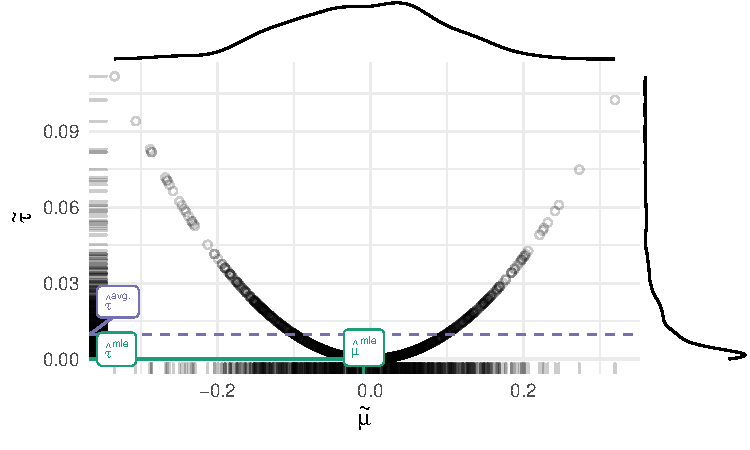
\includegraphics[width=.85\linewidth]{figs/intuition-1.pdf}
  \caption{Simulation 1 of 1,000}
  \label{fig:int1}
\end{subfigure}%
\begin{subfigure}{.5\textwidth}
  \centering
  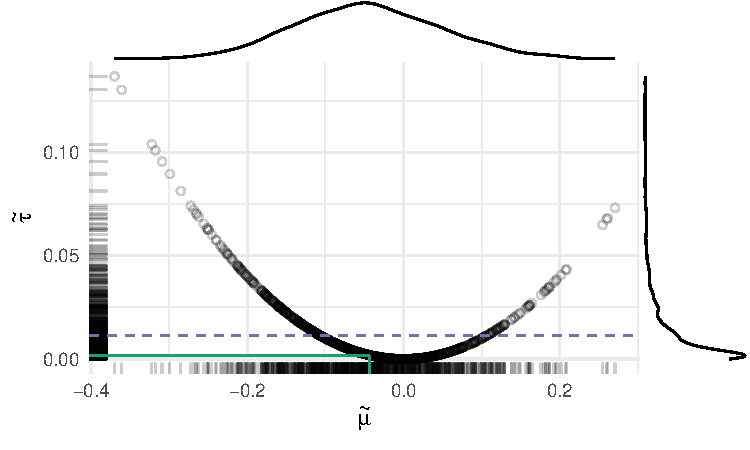
\includegraphics[width=.85\linewidth]{figs/intuition-2.pdf}
  \caption{Simulation 2 of 1,000}
  \label{fig:int2}
\end{subfigure}
\begin{subfigure}{.5\textwidth}
  \centering
  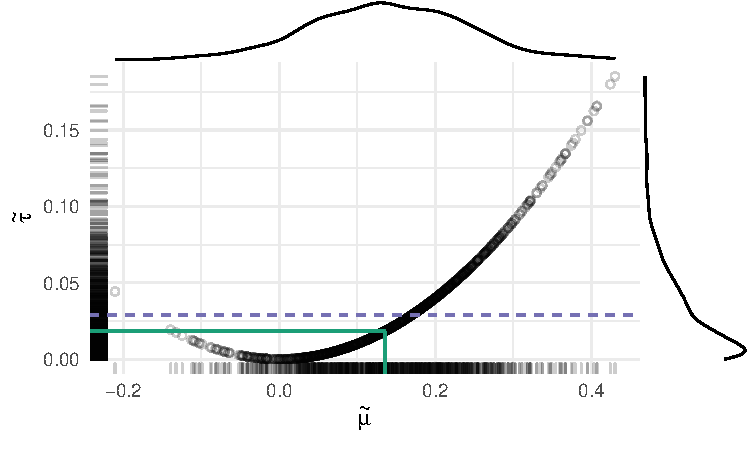
\includegraphics[width=.85\linewidth]{figs/intuition-3.pdf}
  \caption{Simulation 3 of 1,000}
  \label{fig:int3}
\end{subfigure}%
\begin{subfigure}{.5\textwidth}
  \centering
  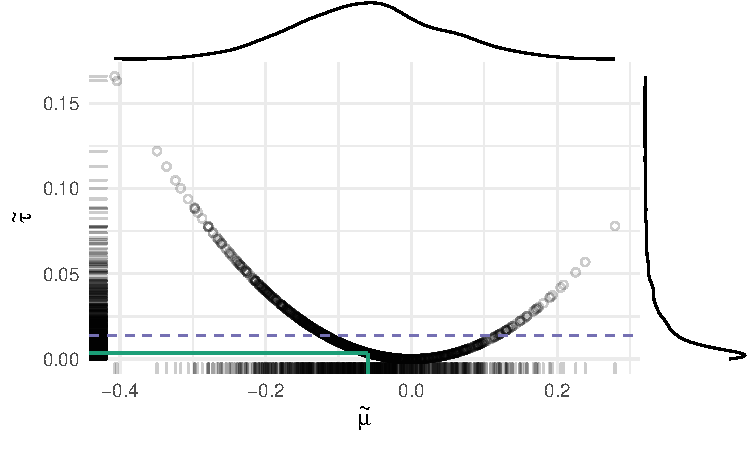
\includegraphics[width=.85\linewidth]{figs/intuition-4.pdf}
  \caption{Simulation 4 of 1,000}
  \label{fig:int4}
\end{subfigure}

\vspace{.1in}
\caption{These four figures illustrate the relationship between $\hat{\tau}^\text{mle}$ and $\hat{\tau}^\text{avg}$ described by Lemma \ref{lem:direction} and Theorem \ref{thm:direction}.}
\label{fig:int}
\end{figure}

Second, to find $\hat{\tau}^\text{mle}$, we simply transform $\hat{\mu}^\text{mle}$ directly using $\hat{\tau}^\text{mle} = \left( \hat{\mu}^\text{mle} \right) ^2$.
The solid green lines show this transformation.
Notice that $\hat{\tau}^\text{mle}$ corresponds approximately to the mode of the density plot of $\tilde{\tau}$ along the right side of the plot, which falls closer to the true value $\tau(0) = 0$ than $\hat{\tau}^\text{avg}$.
The convex transformation $\tau(\cdot)$ has the effect of lengthening the right tail of the distribution of $\tilde{\tau}$, pulling the average well above the mode.
This provides the basic intuition for Lemma \ref{lem:direction}.

Figures \ref{fig:int2}--\ref{fig:int4} repeat this process with three more random samples.
In each sample, the story is similar \textemdash{} the convex transformation stretches the distribution of $\tilde{\tau}$ to the right, which pulls $\hat{\tau}^\text{avg}$ above $\hat{\tau}^\text{mle}$.

We repeat this process 1,000 times to produce 1,000 estimates $\hat{\mu}^\text{mle}$, $\hat{\tau}^\text{mle}$, and $\hat{\tau}^\text{avg}$.
Figure \ref{fig:int-samp} shows the density plots for the 1,000 estimates (i.e., the sampling distributions of $\hat{\mu}^\text{mle}$, $\hat{\tau}^\text{mle}$, and $\hat{\tau}^\text{avg}$).
As we know analytically, $\hat{\mu}^\text{mle}$ is unbiased with a standard error of $\frac{1}{\sqrt{n}} = \frac{1}{\sqrt{100}} = \frac{1}{10}$.
Both $\hat{\tau}^\text{mle}$ and $\hat{\tau}^\text{avg}$ are biased upward, but $\hat{\tau}^\text{avg}$ is biased more.
Theorem \ref{thm:direction} shows why this must be the case.

\begin{figure}[h]
\begin{center}
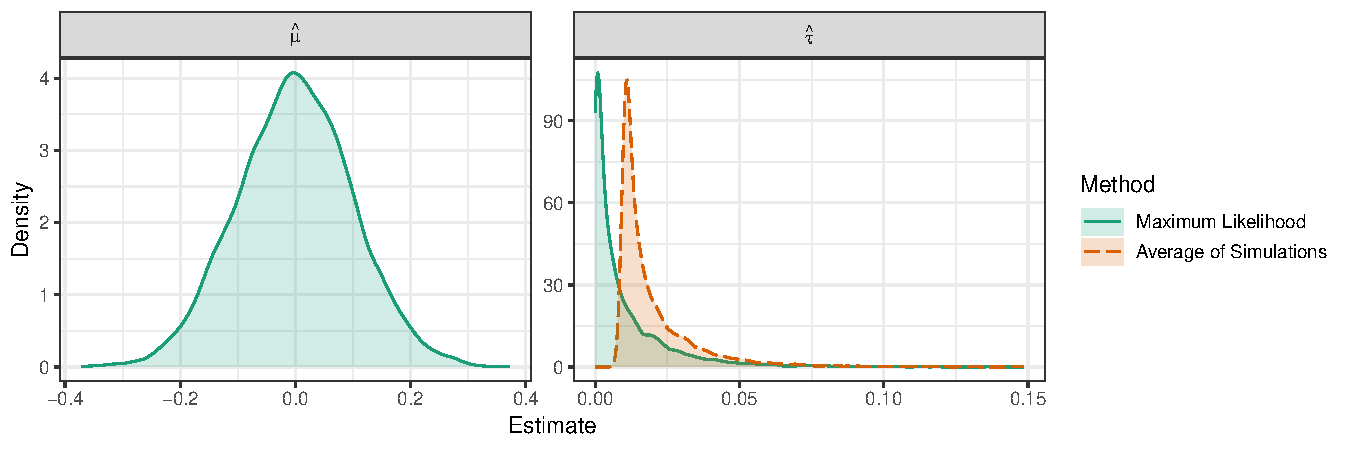
\includegraphics[scale = 0.75]{figs/intuition-sampling.pdf}\\
\vspace{.1in}
\caption{The sampling distributions of $\hat{\beta}^\text{mle}$, $\hat{\tau}^\text{mle}$, and $\hat{\tau}^\text{avg}$.}\label{fig:int-samp}
\end{center}
\end{figure}

\subsection*{Using the Law of Iterated Expectations}

We can also develop the intuition behind our argument analytically via the law of iterated expectations.
For this it helps to alter the notation slightly, making two implicit dependencies explicit. We explain each change below and use the alternate, more expansive notation only in this section.

The law of iterated expectations states that $\E_Y \left( \E_{X \mid Y}(X \mid Y) \right) = \E_X(X)$, where $X$ and $Y$ represent random variables.
The three expectations occur with respect to three different distributions: $\E_Y$ denotes the expectation w.r.t.\@ the marginal distribution of $Y$, $\E_{X \mid Y}$ denotes the expectation w.r.t.\@ the conditional distribution of $X \mid Y$, and $\E_X$ denotes the expectation w.r.t.\@ the marginal distribution of $X$.

Outside of this section, we realize that the distribution of $\tilde{\beta}$ depends on $\hat{\beta}^\text{mle}$ and could be written as $\tilde{\beta} \mid \hat{\beta}^\text{mle}$.
To remain consistent with previous work, especially \cite{KingTomzWittenberg2000} and \cite{Herron1999}, we simply use $\tilde{\beta}$ to represent $\tilde{\beta} \mid \hat{\beta}^\text{mle}$.
The definition of $\tilde{\beta}$ makes this usage clear.
In this section only, we use $\tilde{\beta} \mid \hat{\beta}^\text{mle}$ to represent the conditional distribution of $\tilde{\beta}$ and $\tilde{\beta}$ to represent the \underline{un}conditional distribution of $\tilde{\beta}$.
Intuitively, one might imagine (1) generating a data set $y$, (2) estimating $\hat{\beta}^\text{mle}$, and (3) simulating $\tilde{\beta} \mid \hat{\beta}^\text{mle}$.
If we do steps (1) and (2) just once, but step (3) repeatedly, we have a sample from the conditional distribution $\tilde{\beta} \mid \hat{\beta}^\text{mle}$.
If we do steps (1), (2), and (3) repeatedly, then we have a sample from the \underline{un}conditional distribution $\tilde{\beta}$.
The unconditional distribution helps us understand the nature of the simulation-induced $\tau$-bias.

Applying the law of iterated expectations, we obtain $\E_{\tilde{\beta}} \left( \tilde{\beta} \right) = \E_{\hat{\beta}^\text{mle}}\left( \E_{\tilde{\beta} \mid \hat{\beta}^\text{mle}} (\tilde{\beta} \mid \hat{\beta}^\text{mle}) \right)$.
The three identities below connect the three key quantities from Theorem \ref{thm:direction} to three versions of $\E_{\hat{\beta}^\text{mle}}\left( \E_{\tilde{\beta} \mid \hat{\beta}^\text{mle}} (\tilde{\beta} \mid \hat{\beta}^\text{mle}) \right)$, with the transformation $\tau(\cdot)$ applied at different points.

\begin{alignat}{2}
 \color{color1} \tikzmark{MarkA}\tau \left[ \normalcolor \E_{\hat{\beta}^\text{mle}}\left( \E_{\tilde{\beta} \mid \hat{\beta}^\text{mle}} \left( \tilde{\beta} \mid \hat{\beta}^\text{mle} \right) \right) \color{color1} \right] \normalcolor =&  \tau \left[ \E_{\tilde{\beta}} \left( \tilde{\beta} \right) \right] = \tau \left[\E \left( \hat{\beta}^\text{mle} \right) \right]\text{,} \label{eqn:true}\\
 \E_{\hat{\beta}^\text{mle}}\left( \color{color1} \tikzmark{MarkB}\tau\tikzmark{MarkC} \left[ \normalcolor \E_{\tilde{\beta} \mid \hat{\beta}^\text{mle}} \left( \tilde{\beta} \mid \hat{\beta}^\text{mle} \right) \color{color1} \right] \normalcolor \right)  =&  \E_{\hat{\beta}^\text{mle}} \left( \tau \left[\hat{\beta}^\text{mle} \right] \right) =  \E_{\hat{\beta}^\text{mle}} \left(\hat{\tau}^\text{mle} \right) \text{, and} \justif{\quad}{$\longleftarrow~$ Switch $\tau$ and an $\E$ once.} \label{eqn:mle}\\
\E_{\hat{\beta}^\text{mle}}\left( \E_{\tilde{\beta} \mid \hat{\beta}^\text{mle}} \left( \color{color1} \tikzmark{MarkD}\tau \left[ \normalcolor \tilde{\beta} \mid \hat{\beta}^\text{mle} \color{color1} \right] \normalcolor \right) \right)  =&
\E_{\tilde{\beta}} \left( \tau \left[\tilde{\beta} \right] \right)  =
\E_{\tilde{\beta}} \left(\hat{\tau}^\text{avg} \right) \text{.}\justif{\quad}{$\longleftarrow~$ Switch $\tau$ and an $\E$ again.}\label{eqn:avg}\DrawBox{red}{blue}
\end{alignat}

If we subtract Equation \ref{eqn:mle} from Equation \ref{eqn:true} we obtain the transformation-induced $\tau$-bias in $\hat{\tau}^\text{mle}$ (see Equation \ref{eqn:ti-bias} for the definition of transformation-induced $\tau$-bias).
To move from Equation \ref{eqn:true} to Equation \ref{eqn:mle} we must swap $\tau(\cdot)$ with an expectation once.
This implies that, if $\tau(\cdot)$ is convex, Equation \ref{eqn:mle} must be greater than Equation \ref{eqn:true}.
This, in turn, implies that the bias is positive.

To obtain the $\tau$-bias in $\hat{\tau}^\text{avg}$ we must subtract Equation \ref{eqn:avg} from Equation \ref{eqn:true}.
But to move from Equation \ref{eqn:true} to Equation \ref{eqn:avg} we must swap $\tau(\cdot)$ with an expectation \emph{twice}.
Again, if $\tau(\cdot)$ is convex, then Equation \ref{eqn:avg} must be greater than Equation \ref{eqn:true}.
However, because we expect $\hat{\beta}^\text{mle}$ and $\tilde{\beta} \mid \hat{\beta}^\text{mle}$ to have similar distributions, we should expect the additional swap to roughly double the bias in $\hat{\tau}^\text{avg}$ compared to $\hat{\tau}^\text{avg}$. It is this additional swap that leads to simulation-induced $\tau$-bias.

\section*{Illustrations}

We illustrate simulation-induced $\tau$-bias in three ways: (1) by computing the coefficient-, transformation-, and simulation-induced $\tau$-bias for a simple Poisson regression model, (2) by repeating that exercise for a more complex logistic regression model, and (3) by replicating a published article to show that different estimates result from using the invariance property and averaging simulation draws, respectively, to compute quantities of interest.


\subsection*{Marginal Effects in Poisson Regression}

As a first illustration, consider the Poisson regression model $y_i \sim \text{Poisson}(\lambda_i)$, where $\lambda_i = e^{(-2 + x_i)}$ for $i \in \{1, 2,\ldots, 100\}$.
To create $x_i$, we take $100$ i.i.d.\@ draws from a standard normal distribution.
Assume that the researcher wants to estimate the marginal effect of $x$ on $\E(y)$, so that $\tau(\beta) = \frac{d \E (y)}{dx} = e^{(\beta_{cons} + \beta_x x)}$ for $x$ ranging from $-3$ to $+3$.

We generate 10,000 data sets and use each data set to estimate $\hat{\tau}^\text{mle}$ and $\hat{\tau}^\text{avg}$.
Note that the transformation is convex, so according to Theorem \ref{thm:direction} the $\tau$-bias in both $\hat{\tau}^\text{mle}$ and $\hat{\tau}^\text{avg}$ should be positive.
The rule of thumb suggests about twice as much bias in $\hat{\tau}^\text{avg}$ as in $\hat{\tau}^\text{mle}$.

\begin{figure}[h!]
\begin{center}
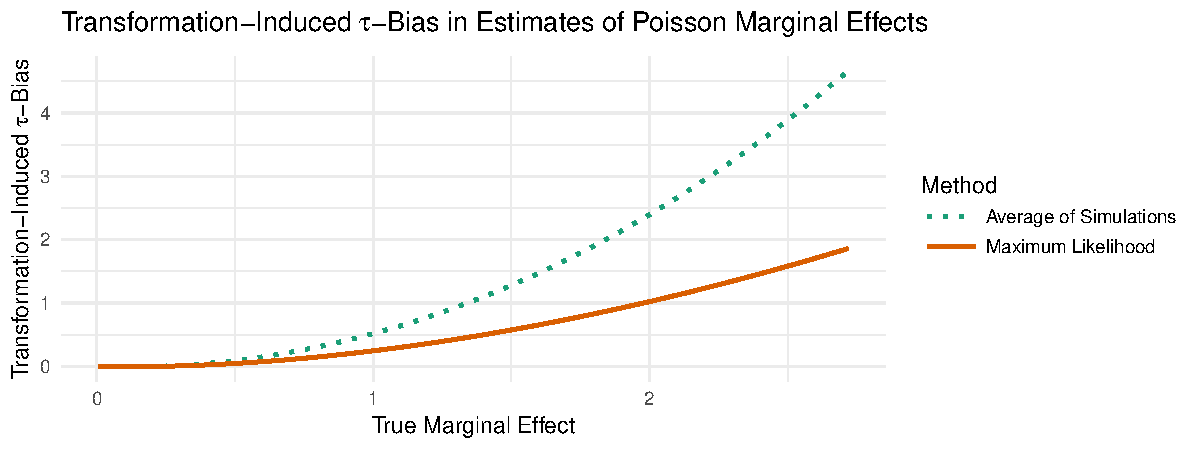
\includegraphics[scale = 0.65]{figs/poisson-mcs.pdf}
\vspace{.1in}
\caption{The figure shows bias in estimates of the marginal effect in a Poisson regression model.
Note that the convex transformation $\tau(\beta) = \frac{d \E (y)}{dx} = e^{(\beta_{cons} + \beta_x x)}$ creates a positive bias (see Theorem \ref{thm:direction}) and that the bias in $\hat{\tau}^\text{avg}$ is about twice as large as the bias in $\hat{\tau}^\text{mle}$ (compare Equations \ref{eqn:avg-approx} and \ref{eqn:mle-approx}).}\label{fig:poisson-mcs}
\end{center}
\end{figure}

Figure \ref{fig:poisson-mcs} shows the $\tau$-bias in $\hat{\tau}^\text{avg}$ and $\hat{\tau}^\text{mle}$ (vertical axis) compared to the true value $\tau(\beta)$ (horizontal axis).
Notice three features of this plot.
First, note that the bias occurs in the expected direction.
Because the transformation $\tau(\beta) = \frac{d \E (y)}{dx} = e^{(\beta_{cons} + \beta_x x)}$ is convex, the bias is positive.
Second, the bias can be substantial, depending on the size of the true marginal effect.
For example, when the true marginal effect equals $1$ the average  $\tau$-bias in $\hat{\tau}^\text{mle}$ is about $.25$ while the $\tau$-bias in $\hat{\tau}^\text{avg}$ is about $.5$.
Third, note that over much of the range of the horizontal axis, the bias in $\hat{\tau}^\text{avg}$ is about twice as large as the bias in $\hat{\tau}^\text{mle}$, as the rule of thumb suggests.

%% perhaps it would be useful to add an additional curve to the plot showing the bias of the simulation-based approach divided by the bias of the ML estimator?

\subsection*{First Differences in a Logistic Regression Model}

As a more realistic example we compute the $\tau$-bias for a more complex logistic regression model.
To find a plausible data-generating process and realistic set of explanatory variables, we base our Monte Carlo study on the classic example of the decision to vote (\citealt{WolfingerRosenstone1980, Nagler1994, HuangShields2000, BerryDeMerittEsarey2010}).
In particular, Berry, DeMeritt, and Esarey (2010) uses a large data set with about 100,000 observations to estimate their models.
We take borrow the coefficients and explanatory variables from Berry, DeMeritt, and Esarey (2010) to use as the data-generating process and explanatory variables, respective, in our Monte Carlo study.

For the data-generating process, we use the model specification and coefficients that \cite{BerryDeMerittEsarey2010} reports in Table 1, Column 2.
To generate the explanatory variables, we randomly draw samples of $100$, $200$, $400$, and $800$ observations from the data that \cite{BerryDeMerittEsarey2010} uses to fit their model.
(Across the Monte Carlo simulations, we generate a new, random outcome variable using these explanatory variables and Berry, DeMeritt, and Esarey's coefficients.)

For the quantity of interest, we focus on the change in the probability of turning out to vote if the election registration deadline occurs $10$ days sooner (a one standard deviation change).
However, the effect of this 10-day shift (and the coefficient-, transformation-, and simulation-induced bias) depends on the original closing date as well as the values of the other explanatory variables.
To capture and present this heterogeneity, we estimate the coefficient-, transformation-, and simulation-induced bias for 250 randomly-chosen observations from the full data.

%\begin{table}[h]
%\begin{center}
%\caption{Logistic regression coefficient estimates reported by Berry, DeMeritt, and Esarey (2010).}
%\begin{tabular}{l D{.}{.}{6.5} }
%\toprule
%closing date           & -0.008 \\
%education              & 0.182  \\
%education$^2$          & 0.012  \\
%age                    & 0.070  \\
%age$^2$                & -0.001 \\
%South                  & -0.116 \\
%gubernatorial election & 0.003  \\
%constant               & -2.523 \\
%\bottomrule
%\end{tabular}
%\label{tab:coef}
%\end{center}
%\end{table}

\begin{figure}[h!]
\begin{center}
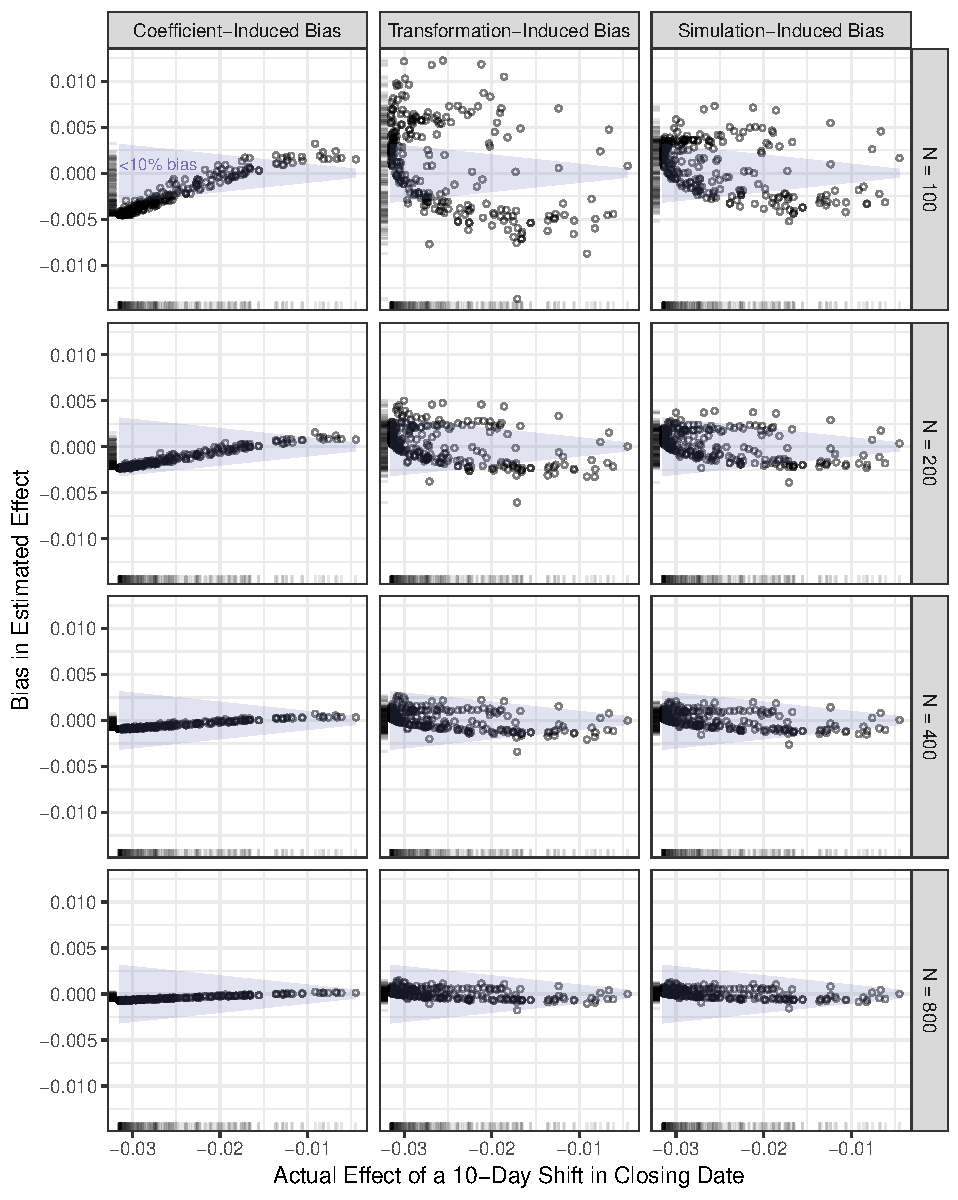
\includegraphics[scale = 0.75]{figs/nagler-fd-bias.pdf}\\
\vspace{.1in}
\caption{The figure shows the coefficient-induced, transformation-induced, and simulation-induced $\tau$-biases for a logistic regression model based on \cite{BerryDeMerittEsarey2010}.
The points the fall outside the orange lines have bias greater than $10\%$.
The numbers at the top right corner of each plot report the average absolute bias across all 250 observations.}\label{fig:nagler}
\end{center}
\end{figure}

Figure \ref{fig:nagler} shows the resulting coefficient-, transformation-, and simulation-induced $\tau$-biases (columns) for the four different sample sizes (rows).
Each point shows the bias for one of the 250 observations. (Remember that the true effect, as well as the size of each type of bias, varies across observations).
First, note that the simulation-induced $\tau$-bias (right-hand column) has a magnitude similar to the well-known small sample bias in logistic regression coefficients (left-hand column).
The magnitude of the simulation-induced $\tau$-bias is similar to the magnitude of the transformation-induced $\tau$-bias (middle column), in line with the approximation we derive in a previous section.
Second, at least in some scenarios, the simulation-induced bias is sufficiently large to meaningfully affect results.
For at least some observations, the simulation-induced bias remains larger than $10\%$ until the sample size exceeds $400$.
Third, while each type of bias disappears asymptotically, the biases disappear at different rates.
Rainey (2017) shows that transformation-induced bias can disappear more slowly than coefficient-induced bias.
We see the same pattern here.
Especially for certain observations, the transformation-induced bias remains large even when the coefficient-induced bias has nearly disappeared.
Consistent with the previous result that simulation-induced bias approximates the transformation-induced bias, we see that the simulation-induced bias disappears more slowly as well.

\subsection*{Replication}

As a final illustration of simulation-induced bias, we replicate an existing study (\citealt{GeorgeEpstein1992}) and compare the ML estimates of quantities of interest (comuted using the invariance property) to simulation average estimate.
We cannot demonstrate bias using this approach (since we do not know the true effects), but we can show that the estimates differ meaningfully.

To unify explanations of U.S. Supreme Court decisions, \cite{GeorgeEpstein1992} fits a single probit model that combines the legal and extralegal models of Court decision-making to a data set of $64$ decisions.
The article models the probability of a conservative decision as a function of whether the Solicitor General filed an Amicus brief (SG = 1) or not (SG = 0) and $10$ other explanatory variables.
See \cite{GeorgeEpstein1992} for details.\footnote{Some readers might be skeptical of this example since the sample size seems clearly insufficient to fit a probit model with $11$ predictors. \citet[3.5.1]{Long1997} recommends a minimum sample size of $100$ observations that for complex models should be increased to at least $10$ observations per parameter. We should point out though that the use of ML estimators with small samples is not uncommon. For example, \cite{Holland2015}, recently published in the \emph{American Journal of Political Science}, fits a Poisson model with 19 observations and 4 predictors.}


We focus on two quantities of interest: the probability of a conservative decision and the effect of the Solicitor General filing a brief, i.e., the first difference in the probability of a conservative decision.
We compute these two quantities of interest for each observation in the data set. Figure \ref{fig:ge} compares the estimates.
First, consider the estimates of the probability of a conservative decision in  Figure \ref{fig:ge1}.
The pattern is clear: when the fitted probability of a conservative decision is less than $50\%$, the simulation average estimate is larger than the ML estimate.
In this region, the transformation (the normal cdf) is convex, leading to positive bias.
When the fitted probability of a conservative decision is greater than $50\%$, the simulation average estimate is smaller than the ML estimate.
In this region, the transformation is concave, causing the bias to be negative.
When the fitted probability of a conservative decision is close to $50\%$, the differences between the two estimates are smaller since the transformation is close to linear in this area.
The same is true for fitted probabilities close to $0\%$ and $100\%$.

Second, note that some of the differences between the estimates are quite large.
For example, when the ML estimates are around $5\%$, the simulation average estimate comes in at about $10\%$.
This difference may seem small at first (i.e., only $5$ percentage points), but for such observations $\hat{\tau}^\text{avg}$ is about twice as large as $\hat{\tau}^\text{mle}$.

Figure \ref{fig:ge2} displays estimates of the effect of the Solicitor General filing an Amicus brief.
The largest differences between the two estimators appear in the upper-right corner of the plot.
For this group of observations, the simulation average estimate suggests that a brief from the Solicitor General increases the probability of a conservative decision by about $40$ percentage points.
The ML estimate on the other hand suggests an increase of about $60$ percentage points.
This difference is certainly meaningful \textemdash{} the maximum likelihood estimate is $50\%$ larger than the estimate based on stochastic simulation.

%Table \ref{tab:ge-qi} summarizes these quantities of interest.

%\begin{table}[h!]
%\centering
%\caption{This table provides the details of the quantities of interest from George and Epstein's (1992) model of U.S. Supreme Court decisions.}
%\label{tab:ge-qi}
%\footnotesize
%\begin{tabular}{@{} m{5cm} m{4cm} m{2.5cm}m{4cm}@{}}
%\toprule
%Description                                                                       & Notation                                                  & Change in Key Explanatory Variable               & Values for Other Explanatory Variables \\ \midrule
%probability of a conservative decision                                            & $\tau(\beta) = \Phi(X_c \beta)$                           & none                                             & every observed combination   \\\hline
%effect of a Solicitor General brief on the probability of a conservative decision & $\tau(\beta) = \Phi(X_\text{high} \beta) - \Phi(X_\text{low}\beta)$ & for $X_\text{high}$, SG = 1, and for $X_\text{low}$, SG = 0 & every observed combination   \\ \bottomrule
%\end{tabular}
%\end{table}

\begin{figure}[h!]
\begin{subfigure}{.5\textwidth}
  \centering
  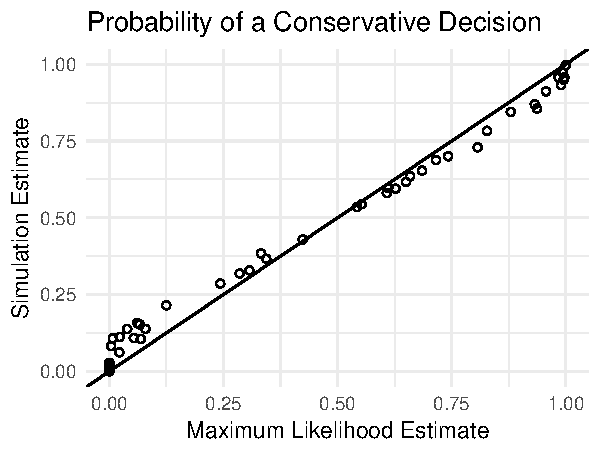
\includegraphics[width=.8\linewidth]{figs/ge-pr.pdf}
  \caption{}
  \label{fig:ge1}
\end{subfigure}%
\begin{subfigure}{.5\textwidth}
  \centering
  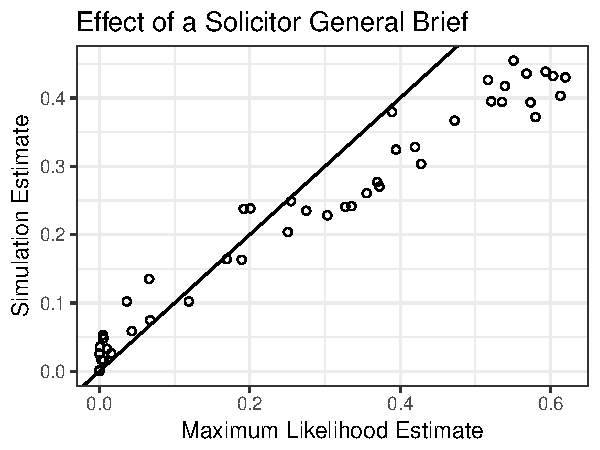
\includegraphics[width=.8\linewidth]{figs/ge-fd.pdf}
  \caption{}
  \label{fig:ge2}
\end{subfigure}
\caption{The figure shows the relationship between the simulation average and the maximum likelihood estimate for two quantities of interest.
The left panel (a) shows the probability of a conservative decision.
The right panel (b) shows the effect of a brief by the Solicitor General on the probability of a conservative decision.}
\label{fig:ge}
\end{figure}

\section*{A Note on \cite{HanmerKalkan2013}}

\cite{HanmerKalkan2013} suggests that researchers avoid the {\it average-case} approach to developing quantities of interest and instead use the and the {\it observed-value} approach.
With either approach, researchers estimate the quantity of interest as a key explanatory variable changes its value.
However, in non-linear models researchers must also deal with the other explanatory variables in the model, because these variables alter the quantity of interest.
The average-case approach sets the other explanatory variables to central values such as the mean, median, or mode.
\cite{HanmerKalkan2013}, in contrast, suggests estimating the quantity of interest for all sample observations, leaving the explanatory variables except for the key variable of interest at their observed values, and then averaging the estimates across the sample.
Here, our notation captures this choice as part of the transformation $\tau(\cdot)$, so Hanmer and Kalkan's (compelling) argument does not undermine or enhance our own.\footnote{We generally agree with the arguments in favor of the observed-value approach but recommend that researchers plot the distribution of quantities of interest in addition to providing a summary measure such as their average. See \cite{AiNorton2003} for examples.}

Because researchers have not drawn a sharp conceptual distinction between using the simulation average estimate and the ML estimate (computed using the invariance property of ML estimators), \cite{HanmerKalkan2013} does not discuss this choice.
Since it explicitly builds on \cite{KingTomzWittenberg2000}, we interpret \cite{HanmerKalkan2013} as relying on the simulation average estimate when computing quantities of interest.
The replication archive for the article confirms that this is indeed the case.

The important point is this: \cite{HanmerKalkan2013} draws a distinction between the average-case and observed-value approaches to computingquantities of interest.
Our paper draws a distinction between computing estimates of quantities of interest (whether average-case or observed-value based) using invariance properity of ML estimators or using King, Tomz, and Wittenberg's (2000) simulation-based approach.
Regardless of whether researchers use the average-case approach or the observed-value approach, the simulation-based approach leads to estimates that include simulation-induced bias that researchers can easily avoid by relying on the invariance property of ML estimators instead.

\section*{Conclusion}

Many social scientists turn to \cite{KingTomzWittenberg2000}'s seminal article when seeking advice on how to interpret, summarize, and present empirical results.
By highlighting the importance of reporting substantively meaningful quantities of interest, it has significantly improved empirical research in political science and neighboring disciplines.
However, political scientists following \cite{KingTomzWittenberg2000}'s advice estimate quantities of interest either with the average of simulated quantities of interest (e.g., Clarify in Stata, Zelig in \texttt{R}) or using the invariance property of ML estimators (e.g., margins in Stata and \texttt{R}).
In practice, researchers' choice between the two approaches seems idiosyncratic rather than principled, depending on their preferred software package rather than statistical principles.
Even the methodological literature fails to pay attention to differences between the two approaches to estimating quantities of interest.

\cite{Rainey2017} stresses the importance of transformation-induced bias, which originates in the non-linear transformation of model coefficient estimates into estimated quantities of interest.
As \cite{Rainey2017} shows, such transformation-induced biases are large when standard errors are large or when the transformation of the model coefficients into quantities of interest is highly non-linear.
We show that when researchers use the simulation average to estimate quantities of interest, they roughly double the transformation-induced bias that Rainey (2017) describes.
We refer to this unnecessary bias as ``simulation-induced bias.''
The good news is that the fix is easy: we do not have to use the simulation-based approach to estimate a quantity of interest.
Instead, we can simply plug model coefficients into the transformation to obtain a ML estimate of the quantity of interest.
We recommend that statistical software does this by default.\footnote{Based on communications with Christopher Gandrud, a member of the Zelig Core Team, it appears that Zelig sometimes uses the median of the simulation draws as point estimator (as opposed to the mean). We cannot find any information in the Zelig documentation (Choirat et al.\@ 2017) for when that might happen. Note that the simulation median corresponds to the ML estimate (in expectation) for monotonic transformations. (Even then, simulation introduces Monte Carlo error that the researcher could easily avoid by using the invariance property of ML estimators in the first place.) To see this revisit the previous example where $\tau(\mu) = \mu^2.$ Imagine the best-case scenario in which $\hat{\mu}^\text{mle} = 0$, so that the estimate based on the invariance property is unbiased. Even then simulated draws of the quantity of interest are almost surely greater than zero. Taking either the mean or the median of the simulated draws will result in an estimator with more bias than the ML estimator.}

Finally, if researchers use the invariance property to compute ML estimates of quantities of interest, how should they conduct statistical inference?
Commonly employed approaches include the delta method, stochastic simulation, and the bootstrap (e.g., \cite{EfronTibshirani1993}.
\cite{KrinskyRobb1991} presents some limited Monte Carlo evidence that these approaches lead to similar inferences but a detailed examination of this question is, to the best of our knowledge, still missing from the literature.

\singlespace
\clearpage
\small
\bibliographystyle{apsr_fs}
\bibliography{bibliography.bib}

\end{document}
